% Poster v2 — Capacity Composition Behind the Zhao Effect
% Compile with: pdflatex poster_v2.tex
% Uses Gemini beamerposter theme, red-orange color scheme

\documentclass[final]{beamer}

% ====================
% Packages
% ====================

\usepackage[T1]{fontenc}
\usepackage{lmodern}
\usepackage[size=a0,orientation=landscape,scale=1.0]{beamerposter}
\usetheme{gemini}
\usecolortheme{redorange}
\usepackage{graphicx}
\usepackage{booktabs}
\usepackage{amsmath,amssymb}
\usepackage{microtype}

% ====================
% Lengths
% ====================

\newlength{\sepwidth}
\newlength{\colwidth}
\setlength{\sepwidth}{0.025\paperwidth}
\setlength{\colwidth}{0.3\paperwidth}

\newcommand{\separatorcolumn}{\begin{column}{\sepwidth}\end{column}}

% ====================
% Title
% ====================

\title{Capacity Composition Behind the Zhao Effect:\\
  SAE-Based Decomposition of Language-Reasoning Interference}

\author{Karlo Vrancic \and Anastasia Ahani \and Riley Kong}

\institute{MIT 6.8610 --- Quantitative Methods for Natural Language Processing --- Spring 2026}

% ====================
% Footer
% ====================

\footercontent{
  \href{https://github.com/kvrancic/nlp-project}{github.com/kvrancic/nlp-project}
  \hfill
  MIT 6.8610 --- Spring 2026
  \hfill
  \href{mailto:kvrancic@mit.edu}{kvrancic@mit.edu}}

% ====================
% Body
% ====================

\begin{document}

\begin{frame}[t]
\begin{columns}[t]
\separatorcolumn

% =====================================================================
% COLUMN 1: Setup + Replication
% =====================================================================
\begin{column}{\colwidth}

  \begin{block}{1. Motivation \& Setup}

    \heading{The Zhao paradox}
    Multilingual LLMs reason worse in non-English languages.
    Zhao et al.\ (NeurIPS 2025) showed, counter-intuitively, that
    \emph{removing} language-specific representations \emph{improves}
    reasoning.
    Their method: compute per-language mean hidden states on translated math
    problems, extract a ``language subspace'' via SVD, and project it out at
    inference ($\hat{h} = h - \lambda\, M_s M_s^\top h$).
    Across 10 models (Qwen, DeepSeek) and 10 languages they found consistent
    gains --- up to +12.8pp, largest for low-resource languages.

    \heading{Research question}
    What are these features doing, and what are they encoding?
    Zhao's method operates on entire subspaces and cannot identify individual
    features or explain the mechanism.
    We decompose the effect to \emph{individual SAE features} to characterize
    both the mechanism and the nature of the ablated representations.

    \heading{Setup}
    \begin{itemize}
      \item \textbf{Model:} Gemma 3 4B IT (untested by Zhao)
      \item \textbf{SAEs:} Gemma Scope 2, 16k-width residual, layer 17
      \item \textbf{Data:} MGSM --- 250 math problems $\times$ 5 languages
            (en, zh, es, bn, sw)
      \item \textbf{Feature selection:} intersection of top-$k$ by
            monolinguality ($\nu$) with top-$k$ by language-probe importance
            (``A$\cap$B'')
      \item \textbf{Ablation:} directional QR-orthogonalized projection,
            $k{=}20$ per language
    \end{itemize}

  \end{block}

  \begin{block}{2. Replication: Ablation Improves Reasoning}

    Ablating procedure-selected features at layer 17 reproduces and extends
    the Zhao effect on Gemma 3 4B.

    \begin{center}
    \renewcommand{\arraystretch}{1.15}
    \begin{tabular}{l c c c}
    \toprule
    \textbf{Lang} & \textbf{Baseline} & \textbf{Zhao SVD}
      & \textbf{SAE ablation} \\
    \midrule
    en & 0.580 & 0.632 & \textbf{0.712} \\
    zh & 0.624 & 0.624 & 0.596 \\
    es & 0.568 & 0.600 & \textbf{0.636} \\
    bn & 0.564 & 0.564 & 0.480 \\
    sw & 0.320 & 0.332 & 0.296 \\
    \midrule
    \textbf{Mean} & 0.531 & 0.550 & 0.544 \\
    \bottomrule
    \end{tabular}
    \end{center}

    Mean accuracy under SAE ablation (0.544) is comparable to the Zhao
    baseline (0.550), confirming that individual-feature ablation replicates
    the subspace-level effect.
    SAE ablation outperforms Zhao for English (+8.0pp over Zhao) and Spanish
    (+3.6pp), suggesting feature-level targeting can be more precise than
    subspace projection for some languages.

  \end{block}

\end{column}

\separatorcolumn

% =====================================================================
% COLUMN 2: Mechanism (the positive contribution)
% =====================================================================
\begin{column}{\colwidth}

  \begin{alertblock}{3. Mechanism: Capacity Composition}

    We find direct evidence for \textbf{capacity composition}:
    language-correlated and reasoning-correlated features compete for
    residual-stream bandwidth. Suppressing one class frees the other.

    After ablating the top-20 procedure-selected features at L17, we measure
    activation changes across 21 reasoning-correlated features
    (50 problems $\times$ 5 langs, Wilcoxon signed-rank).

    \begin{figure}
      \centering
      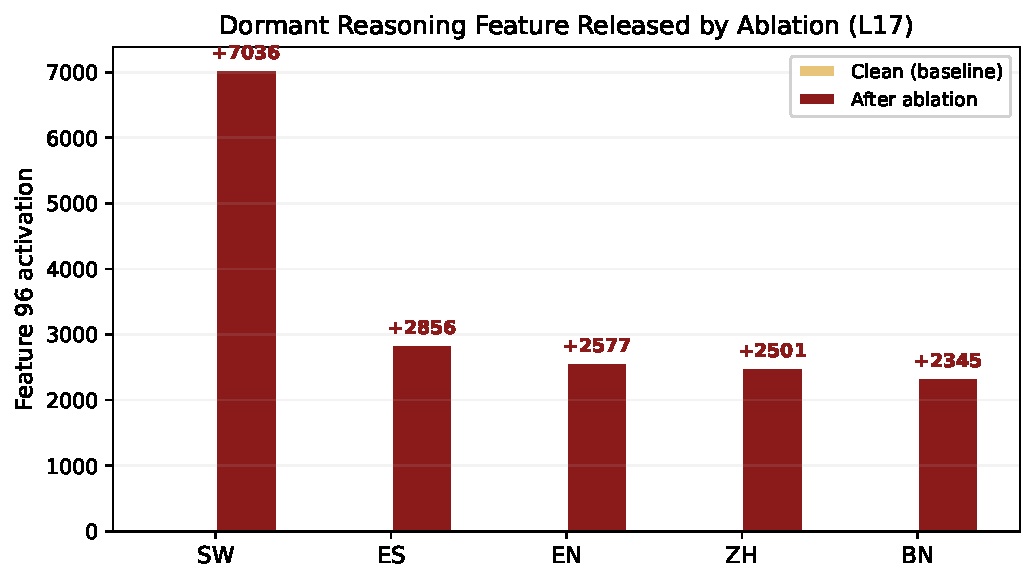
\includegraphics[width=0.70\linewidth]{figures/feat96_dormant.pdf}
      \vspace*{-0.5em}
      \caption{Feature 96: completely dormant at baseline, activates strongly
        (2345--7036) across all languages after ablation.
        All $p < 1.8 \times 10^{-15}$.}
    \end{figure}

    \vspace*{-0.5em}
    \textbf{Dormant $\to$ active:} Feature 96 fires at 2345--7036 across
    all five languages when procedure-selected features are removed ---
    reasoning capacity suppressed by competition.
    \textbf{Active $\to$ suppressed:} Feature 34 collapses from 2177 to 0
    --- space reclaimed.

    Ablation does not destroy capability; it \textbf{reallocates capacity}.
    This reallocation occurs across all five languages, even those where
    overall accuracy does not improve.

  \end{alertblock}

\end{column}

\separatorcolumn

% =====================================================================
% COLUMN 3: What are these features? + Takeaways
% =====================================================================
\begin{column}{\colwidth}

  \begin{block}{4. What Are These Features?}

    The procedure selects features whose ablation reliably triggers capacity
    reallocation.
    But what do these features represent?
    Cross-domain comparison raises questions about whether they are
    ``language features'' in a domain-general sense.

    \heading{Cross-domain feature instability}
    Running the \emph{same} selection procedure (A$\cap$B) on FLORES-200
    (1012 parallel translations, no math content) versus MGSM yields
    substantially different feature sets for every language:

    \begin{figure}
      \centering
      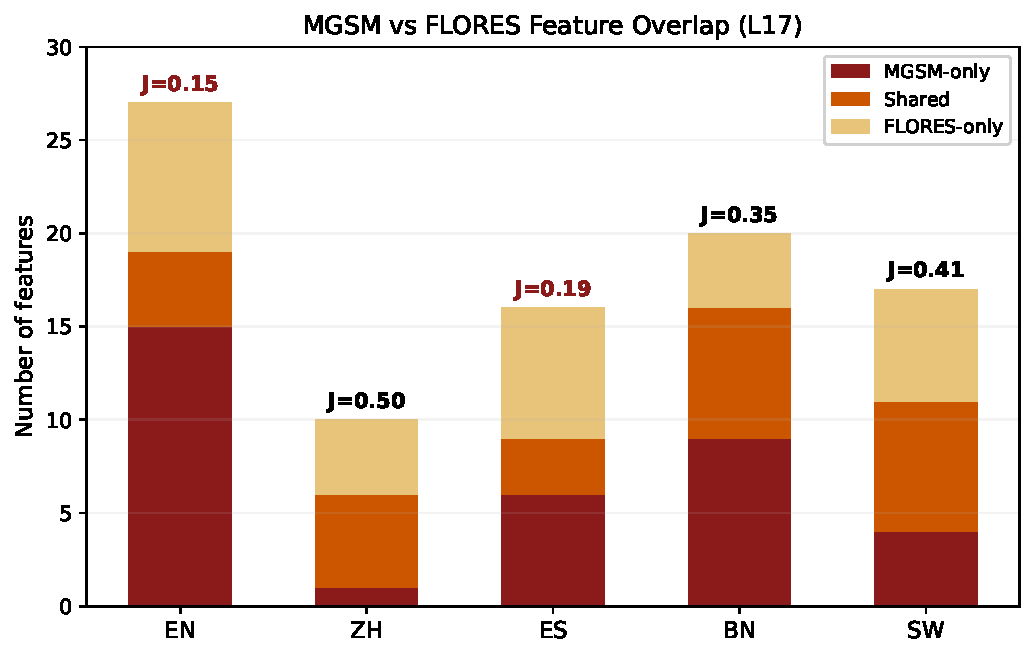
\includegraphics[width=0.82\linewidth]{figures/jaccard_overlap.pdf}
      \vspace*{-0.5em}
      \caption{Per-language overlap between MGSM-derived and FLORES-derived
        procedure-selected features at L17. Jaccard ranges 0.15--0.50;
        every language shows substantial non-overlap.}
    \end{figure}

    The procedure's notion of ``language feature'' is content-dependent:
    the same statistical criteria identify different features when applied
    to math text versus neutral text.
    Even within FLORES alone, the two selection methods (monolinguality and
    probe) agree on only 10--15\% of candidates (Jaccard 0.099--0.149).

    These observations do not invalidate the ablation effect --- the
    mechanism operates regardless.
    But they suggest ``language feature'' as used here is a
    procedure-defined label tied to input content; whether the selected
    features encode language identity in a domain-general sense remains
    an open question.

  \end{block}

  \begin{exampleblock}{5. Takeaways \& Future Work}

    \begin{enumerate}
      \item \textbf{Replication.}
            SAE ablation reproduces the Zhao effect on Gemma 3 4B IT,
            extending the finding beyond Qwen/DeepSeek.

      \item \textbf{Mechanism.}
            Capacity composition: ablation releases dormant reasoning
            features ($\Delta$ up to +7036, $p < 10^{-15}$).

      \item \textbf{Open question.}
            Procedure-selected features are content-dependent
            (Jaccard 0.15--0.50); whether they encode language identity
            in a domain-general sense is unresolved.
    \end{enumerate}

    \heading{Future work}
    Ablate FLORES-derived features on MGSM; extend to additional models;
    causal OOD ablation on language-identification tasks.

    \heading{Limitations}
    {\small
    Single model, single task, 5 languages.
    Global $k{=}20$; per-language $k$ would likely improve results.
    }

    \heading{References}
    {\small
    Zhao et al.\ (NeurIPS 2025);
    Deng et al.\ (2025);
    Bricken et al.\ (2023);
    Lieberum et al.\ (2024)
    }

  \end{exampleblock}

\end{column}

\separatorcolumn
\end{columns}
\end{frame}

\end{document}
